\documentclass[a4paper,12pt]{article}
\usepackage[dutch]{babel}
\usepackage{float}
\usepackage{amsmath}
\usepackage{graphicx}
\usepackage[small,bf,hang]{caption}
\usepackage{subcaption}
\usepackage{wrapfig}
\usepackage[hyphens]{url}
\usepackage[pdftex,bookmarks=true]{hyperref}
\usepackage{fullpage}
\usepackage{listings}
\usepackage[bottom]{footmisc}
\usepackage[none]{hyphenat}
\newcommand{\doekezot}{\\\\\noindent}
\newcommand{\juisteen}{\'{e}\'{e}n }
\renewcommand{\familydefault}{\sfdefault} %zet serif af, arial
\renewcommand{\lstlistingname}{Codefragment}
\sloppy
\lstset{ 
basicstyle=\footnotesize,       
frame = single,
emph={sudo,mkdir,chown,chmod,mv,cp,wget,tar,unzip,mvn},
emphstyle={\bfseries},
breaklines = true
%numbers = left
}
\begin{document}
\noindent
\begin{titlepage}
\begin{center} 
\vspace*{\fill}

\huge{\bf{Projecten 1}} \\ 
\vspace*{1cm}

\hrule
\vspace*{0.3cm}
\huge{Technisch rapport} \\
\vspace*{0.3cm}
\hrule
\vspace*{1cm}

\large{Hans Ott, Alexander Delemarre en Pieter De Bruyne}\\
\large{2e semester 2013-2014}
\vspace*{0.8cm}

%\large{Pieter De Bruyne}

\vspace*{\fill}
\end{center}
\end{titlepage}
\tableofcontents
\newpage

\section{Structuur van de code}

De code van het project is onderverdeeld in 5 mappen.

\begin{itemize}
\item De map Application bevat de code van de Android applicatie.
\item Database bevat het databaseschema en de sqlite databasefile.
\item Hardware bevat de api en de de code die de hardware aanstuurt.
\item Interface bevat de code van de webapplicatie.
\item Pebble bevat de code van de pebble applicatie.
\end{itemize}

\section{Aansluiten van de pi aan de randapparatuur}

\subsection{De MCP23017 chip}

\begin{figure}[ht!]
  \centering
    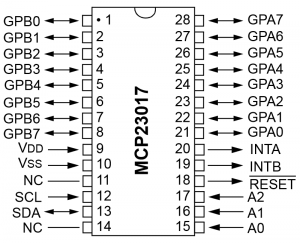
\includegraphics[scale=0.50]{mcp23017.png}
   \caption*{mcp23017}
\end{figure}
\noindent
Het aansluiten van apparaten op de Raspberry Pi gebeurt niet rechtstreeks via de GPIO interface maar met GPIO expander chip
met 16 pinnen. De MCP23017 chip communiceert met de Raspberry Pi via het I2C protocol. De sda en scl lijnen van de chip moeten dus verbonden worden met de Raspberry Pi. Er kunnen 8 chips worden aangesloten op de bus wat het totaal aantal pinnen op 128 brengt.
Elke chip moet een uniek adres krijgen door de 3 adrespinnen aan te sluiten.

\begin{figure}[ht!]
  \centering
    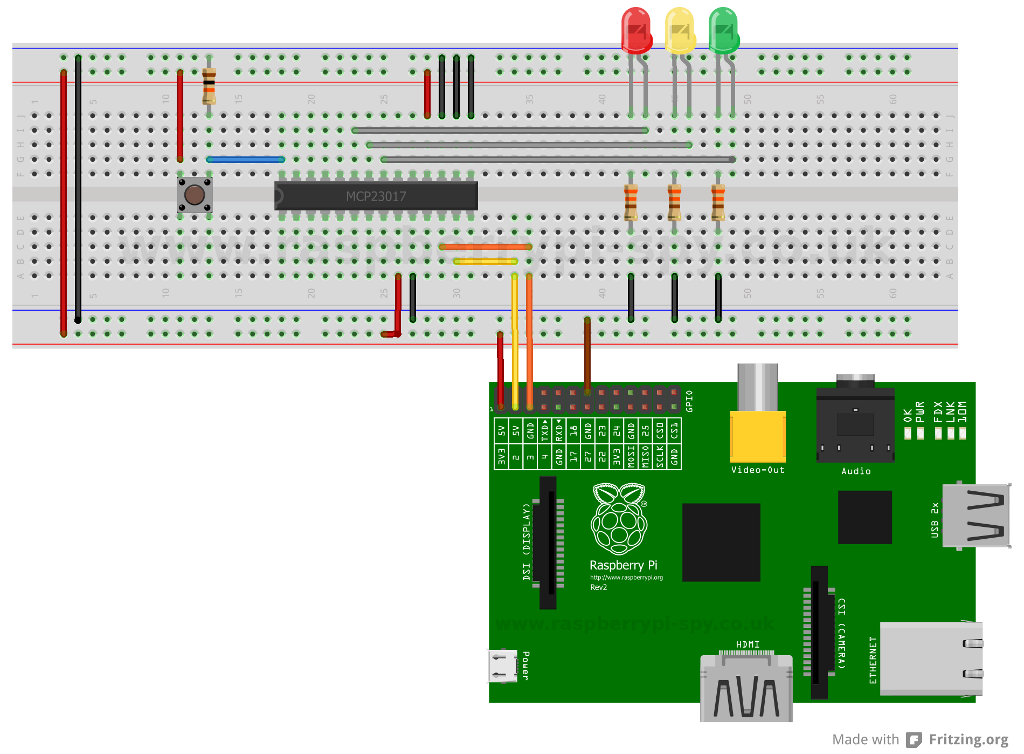
\includegraphics[scale=1.00]{chiptopi.png}
   \caption*{Aansluiten van de i/o expander}
\end{figure}
\noindent
Om te kunnen werken met i2c op de Raspberry Pi moet het commando \texttt{sudo apt-get install i2c-tools}
worden uitgevoerd in de linux omgeving van de RaspberryPi. Om I2C ook werkelijk toe te laten moeten in het bestand \texttt{/etc/modules} volgende 2 lijnen worden toegevoegd :
\begin{itemize}
\item \texttt{i2c-bcm2708}
\item \texttt{i2c-dev}
\end{itemize}
\noindent
Daarnaast moet ook nog I2C uit de blacklist worden gehaald. In het bestand \texttt{/etc/modprobe.d/raspi-blacklist.conf} moeten volgende lijnen in commentaar worden geplaatst.

\begin{itemize}
\item \texttt{\#blacklist spi-bcm2708}
\item \texttt{\#blacklist i2c-bcm2708}
\end{itemize}
\noindent
In de api (die draait in node.js) wordt gebruikt gemaakt van een i2c library. Daarmee kunnen bytes worden verzonden en ontvangen via i2c. De driver die de met de chip communiceert en de juiste registers instelt is zelfgeschreven en zit in het bestand \texttt{icconnection.js}.

\subsection{De temperatuursensor}

Aangezien de RaspberryPi geen A/D converter aan boord heeft maken we gebruik van een temperatuursensor met ingebouwd A/D conversie. De temperatuursensor heeft het typenummer DS18B20 en wordt als volgt aangesloten :

\begin{figure}[ht!]
  \centering
    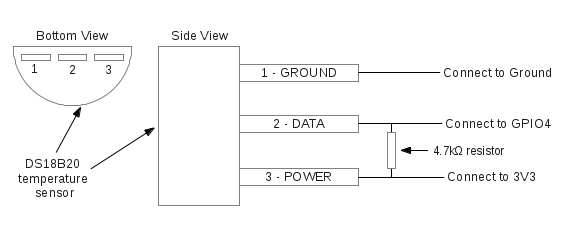
\includegraphics[scale=0.75]{sensor-connection.png}
   \caption*{Aansluiten van de temperatuursensor}
\end{figure}
\noindent
Om de sensor te kunnen uitlezen moeten eerst 2 modules worden geactiveerd: 
\begin{itemize}
\item \texttt{sudo modprobe w1-gpio}
\item \texttt{sudo modprobe w1-therm}
\end{itemize}
\noindent
In de map \texttt{/sys/bus/w1/devices/} zit nu een map met als naam het serienummer van de sensor. Het uitlezen van de temperatuur gebeurt met het openen van het ``bestand'' \texttt{w1\_slave}.
\begin{figure}[ht!]
  \centering
    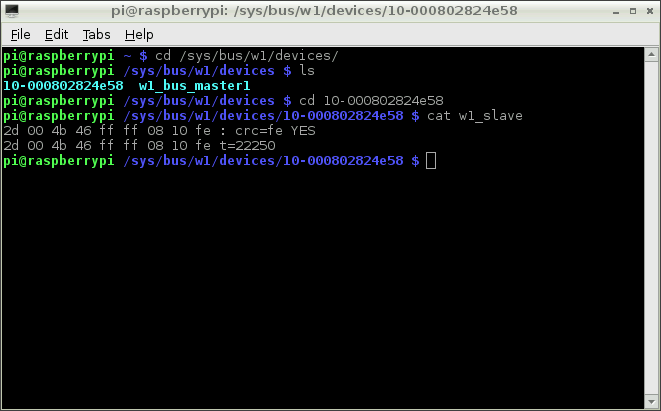
\includegraphics[scale=0.50]{bash-temp-sensor.png}
   \caption*{Uitlezen van de temperatuur}
\end{figure}

\section{Opstarten van de API}
\noindent
De api die het domoticasysteem doet draaien is geschreven in node.js. Het spreekt voor zich dat node ge\"installeerd moet zijn op de RaspberryPi. Verder zijn een aantal node.js pakketten nodig. Deze kunnen worden ge\"installeerd met de npm package manager.
De gebruikte pakketten zijn:

\begin{itemize}
 \item express: een framework voor de basisfunctionaliteit van een webserver
 \item cron: voor het uitvoeren van getimede opdrachten in de achtergrond
 \item sqlite: om met de lokale database te kunnen werken
 \item passport: om een basisbeveiliging mogelijk te maken
\end{itemize}
\noindent
Het opstarten van de api kan met de commando \texttt{sudo node app.js}. Of met het start.sh script. Het is belangrijk dat het node proces root rechten krijgt. De api luistert standaard op poort 8080.


\newpage

\section{Bronnen}

\begin{enumerate}
\item \url{http://www.raspberrypi-spy.co.uk/2013/07/how-to-use-a-mcp23017-i2c-port-expander-with-the-raspberry-pi-part-1/}
\item \url{https://www.cl.cam.ac.uk/projects/raspberrypi/tutorials/temperature/}
\item \url{http://learn.adafruit.com/downloads/pdf/adafruits-raspberry-pi-lesson-11-ds18b20-temperature-sensing.pdf}
\item \url{https://github.com/mapbox/node-sqlite3/wiki/API}
\item \url{http://passportjs.org/}
\item \url{https://www.npmjs.org/package/cron}

\end{enumerate}


\end{document}
